%%% Local Variables:
%%% mode: latex
%%% TeX-master: "../doc"
%%% coding: utf-8
%%% End:
% !TEX TS-program = pdflatexmk
% !TEX encoding = UTF-8 Unicode
% !TEX root = ../doc.tex
Das Resultat besteht wie beschrieben aus verschiedenen Artefakten. In diesem Abschnitt wird konkret auf die Resultate der verschiedenen Schritte eingegangen und der Zusammenhang hergestellt.

\section{LOD Pipeline}

Der Kern der Arbeit stellt die LOD Pipeline, \e{lode} genannt, dar. Dieses Tool liefert eine für das Web optimierte Möglichkeit LOD Artefakte für eine Vielzahl von Anwendungsgebieten zu generieren.

\subsection{Workflow}

Der übliche Ablauf für das generieren von LOD Artefakten ist wie folgt:
Für ein gegebenes Modell werden innerhalb vom Modellierungstool wie z.B. Blender bestimmte LOD Stufen von Hand generiert. Anschliessend werden die verschiedenen Stufen exportiert und manuell in die Applikation integriert. Fine Tuning erfordert so sowohl Anpassungen an den Modellen als auch im Code.

\subsection{lode Pipeline}

Das Ziel von \e{lode} ist es, für ein möglichst breites Spektrum von Anwendungsfällen eine einfache Lösung anzubieten und somit die Hemmschwelle für den Einsatz von LOD Artfakten zu reduzieren.

Deshalb setzt \e{lode} konsequent auf moderne Entwicklungsprozesse, manuelle Schritte sollen auf ein Minimum reduziert werden.

\subsection{lode Ablauf}

Ein Modell wird erstellt und als glTF innerhalb des Projekts gespeichert. Eine zum Modell gehörige Konfigurationsdatei kann mittels \e{CLI} angelegt werden (wie in Abbildung \ref{fig:lodecliconfig} dargestellt) und \e{lode} generiert die darin beschriebenen LOD Artfakte (in Abbildung \ref{fig:lodeclirun} ersichtlich). Wenn sich das Modell oder die Konfiguration anpasst werden die notwendigen Schritte automatisch durchgeführt. So ist es möglich, schnell Anpassungen vorzunehmen und die Änderungen im Projekt zu testen.

\begin{figure}[H]
  \centering
  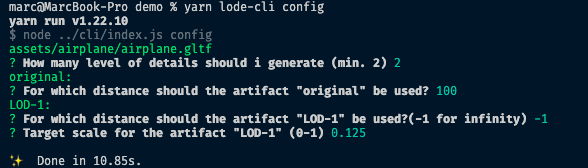
\includegraphics[width=0.8\columnwidth]{resultate/screenshotlodecliconfig.png}
  \caption{lode \e{CLI} config – Konfiguriert die gewünschten LOD-Artefakten}
  \label{fig:lodecliconfig}
\end{figure}

\begin{figure}[H]
  \centering
  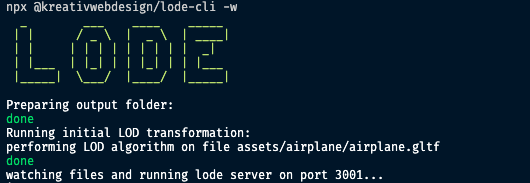
\includegraphics[width=0.8\columnwidth]{resultate/screenshotlodeclirun.png}
  \caption{lode \e{CLI} run – Generiert die gewünschten LOD-Artefakten}
  \label{fig:lodeclirun}
\end{figure}

Die Artfakten können innerhalb der Applikation mithilfe einer Bibliothek geladen werden. Bei Anpassungen an der Konfigurationsdatei werden die neuen Detailstufen automatisch generiert. Das zugehörige \e{lode-ui} (in Abbildung \ref{fig:lodeui} gezeigt) bietet zudem die Möglichkeit die verschiedenen Detailstufen miteinander vergleichen zu können und die Konfiguration möglichst einfach zu justieren.

\begin{figure}[H]
  \centering
  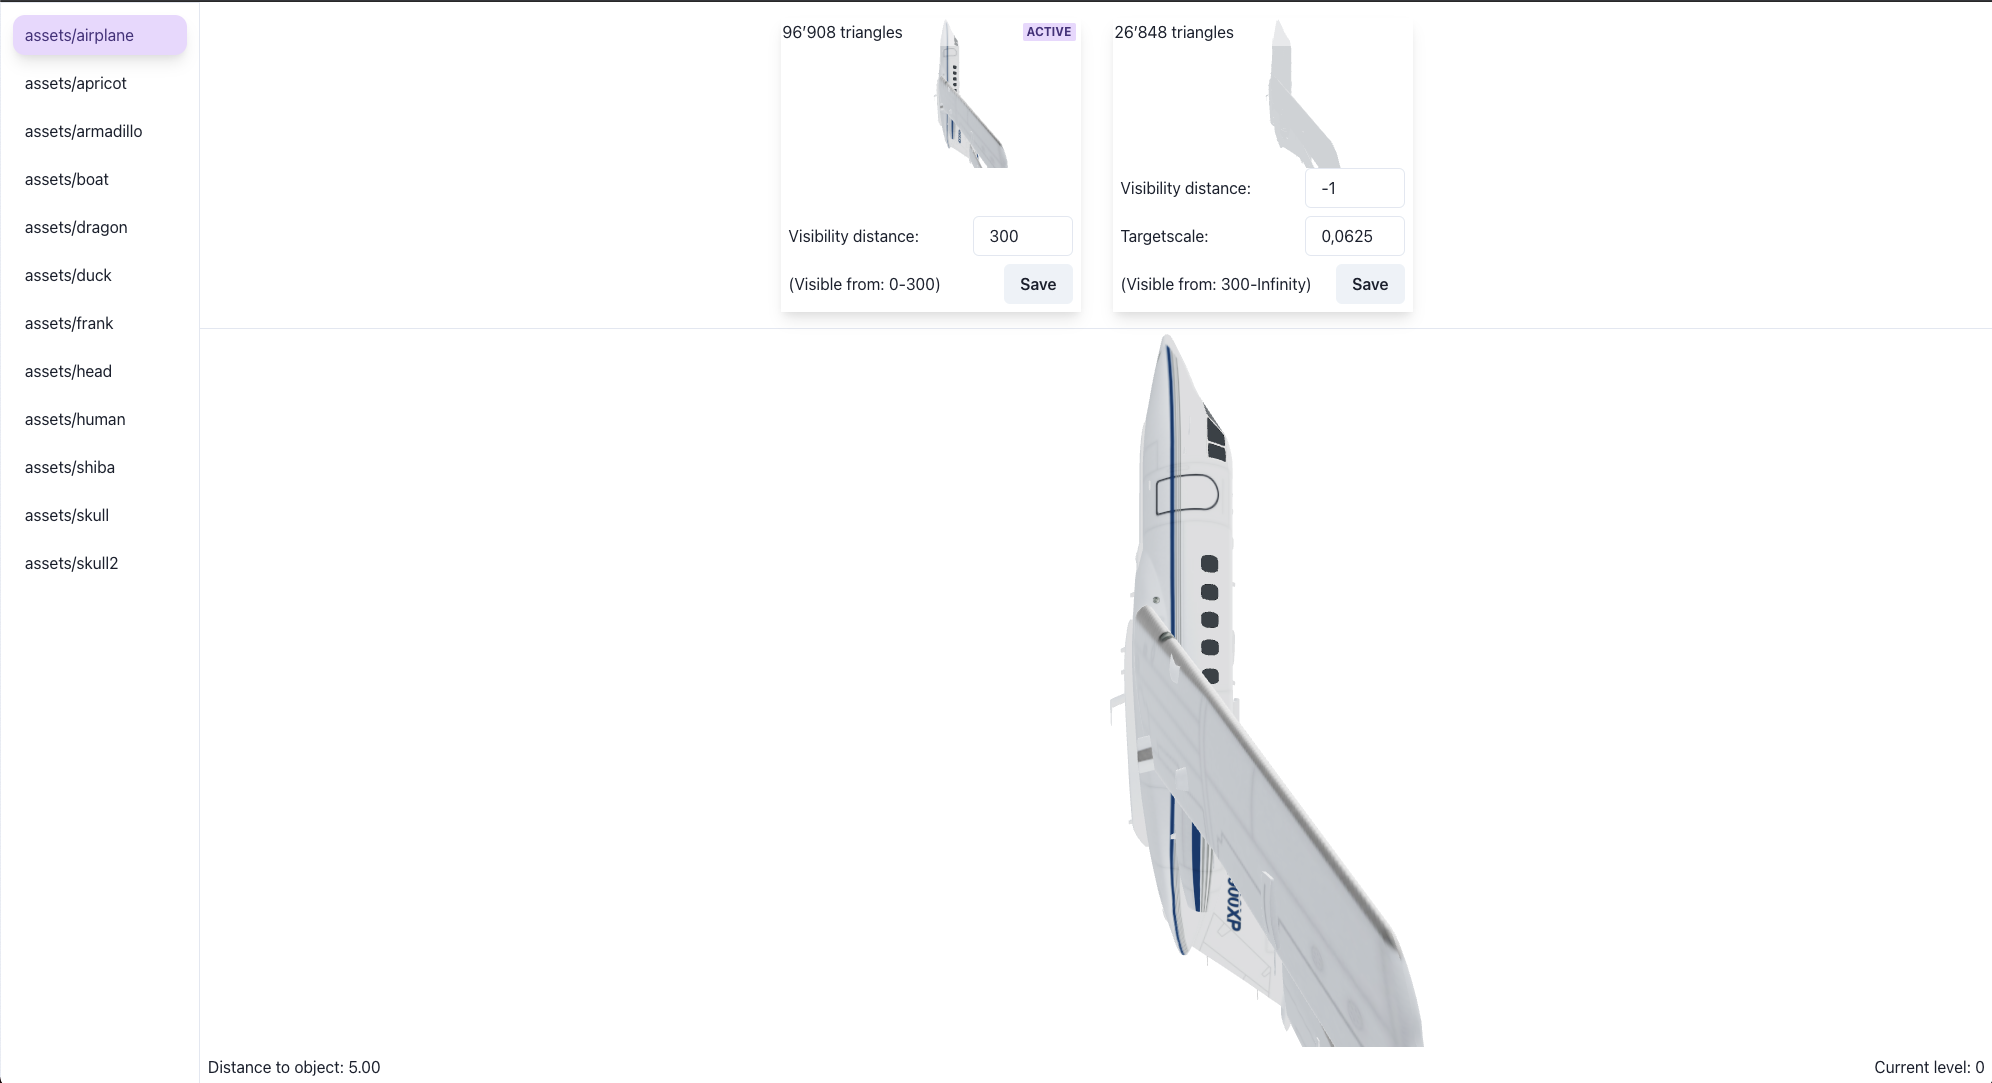
\includegraphics[width=1\columnwidth]{resultate/screenshotlodeui.png}
  \caption{lode-ui}
  \label{fig:lodeui}
\end{figure}

\section{LOD Generierung}

Für das Erstellen von LOD Artefakten wurde ein für LOD Artefakte optimierte Version des in \autoref{chap:surfaceSimplificationAlgorithm} erklärten \e{Surface Simplification Algorithmus} entwickelt.

\subsection{Implementation}

Die Implementation des Algorithmus wurde in JavaScript, basierend auf \fGls{Node.js}{JavaScript Ausführungsumgebung welche ohne einen Browser verwendet werden kann}, umgesetzt. Grund dafür ist das einbinden von \e{lode} in bestehende Entwicklungsabläufe in der Webentwicklung. So ist es einfach möglich das Paket kostenlos mithilfe von \gls{npm} zur Verfügung zu stellen.

\subsection{Artefakte}

Die generierten Artefakte sind unabhängig voneinander. So ist es nicht notwendig alle Artefakte zu jeder Zeit zu laden. Dies hat den primären Vorteil, dass es möglich ist progressives Laden als Erweiterung zuzulassen. Progressives laden bedeutet, dass zuerst die LOD Artefakte mit den wenigsten Details geladen werden und angezeigt werden bis die detaillierteren Level visualisiert werden.
Es ist sogar möglich auf gewissen Geräten die detaillierten Level überhaupt nicht zu laden und so zum Beispiel Bandbreite zu sparen.

\subsection{Texturen}

Bei vielen Modellen sind der grösste Teil der Speichergrösse die Texturen. Das Optimieren der geometrischen Struktur reduziert die zugehörigen Texturen jedoch nicht. Um trotzdem möglichst grosse Einsparungen für die Texturen zu ermöglichen wurde eine Methode entwickelt, welche versucht die prominenteste Farbe eines Modelles zu extrahieren und diese für die Vereinfachungen zu verwenden.
Diese Technik führt zu signifikanten Detailverlusten bei der Nahbetrachtung und ist somit ungeeignet für das Verwenden bei der ersten LOD Stufe. Für alle weiteren Stufen überwiegt jedoch der Vorteil der Vereinfachung im Vergleich zum Detailverlust.

\section{Benchmark}

Das Ziel des Benchmarks ist der Vergleich einer Version ohne Einsatz von LOD und einer Umgebung, welche LODs einsetzt. Um eine möglichst praxisnahe Aussage treffen zu können, wird hierfür eine Demo Szenerie verwendet, welche einer echten Anwendung so nah wie möglich kommt. Somit wird gewährleistet, dass es nicht nur in der Theorie einen Nutzen für LODs gibt, sondern dieser in der Praxis vorhanden ist.

\paragraph{Browser Umgebung}
Um den Umfang des Benchmarks überschaubar zu halten, wurde ausschliesslich ein Benchmark für Google Chrome entwickelt.
Google Chrome basiert auf \fgls{Chromium}{Open Source Browser-Projekt welches von Google entwickelt wird}, dieselbe Engine, welche auch Microsoft Edge oder Opera verwenden.
Einen Benchmark basierend auf Google Chrome liefert somit auch Indizien für diese beiden Browser, auch wenn gewisse Abweichungen möglich sind.
Neben dem Marktführer Chrome sind Mozilla Firefox oder Safari von Apple ebenfalls Optionen. Jedoch wurde primär aufgrund des Marktanteils von total rund 70\% \cite{browserUsage} zugunsten von Google Chrome entschieden.
Die getroffenen Aussagen bezüglich Laufzeitverhalten behalten ihre Gültigkeit auch für andere Browser.

\paragraph{Automation}
Um die Tests durchzuführen, wird ein Testautomationstool benötigt; unter anderem der Einsatz von Selenium wurde in Erwägung gezogen.
Der Vorteil von Selenium ist insbesondere, dass der Benchmark für weitere Browser ausgeweitet werden könnte.
Da jedoch das Analysieren der GPU Daten stark vom System abhängig ist und dafür zusätzliche Komplexität notwendig wäre, wird in diesem Benchmark die im Google Chrome integrierten \e{Chrome DevTools} eingesetzt.
Selenium bietet zurzeit eine suboptimale Integration für das \e{Chrome DevTools Protocol}.
Um mögliche Diskrepanzen zwischen Systemen möglichst gering zu halten, wurde jedoch entschieden, auf die bewährte Lösung von Google Chrome zu setzen.
\fgls{Puppeteer}{Node.js Library, die eine API anbietet zum Steuern von \gls{Chromium} oder Chrome über das Chrome DevTools Protocol}, eine weitere Option für die Automation, ist eine Bibliothek, die eine vereinfachte Schnittstelle zu einer Chromium Instanz bietet.
Sie wird zudem direkt von Google entwickelt und bietet somit eine stabile Grundlage zur Kommunikation mit den \e{Chrome DevTools}.

\paragraph{Profiling}
Die \e{Chrome DevTools} erlauben es, ein detailliertes Laufzeitprofil einer Applikation anzulegen.
Im Profil befinden sich Informationen zu CPU- und GPU-Auslastung, aber auch generelle Informationen bzgl. der \gls{Rendering Engine} werden gesammelt.
Die Analyse dieser Daten ermöglicht es, eine Aussage zum Laufzeitverhalten einer Applikation zu tätigen.

\paragraph{Testaufbau}
Derselbe Testablauf wird sowohl für die optimierte als auch für die unoptimierte Version verwendet.
Bei einem Testablauf werden folgende Schritte durchlaufen:

\begin{enumerate}
  \item Öffne die Applikation in einer \emph{Chromium} Instanz.
  \item Warte bis die Seite geladen ist.
  \item Starte das \emph{Profiling}.
  \item Warte $n$ Sekunden.
  \item Stoppe das \emph{Profiling}.
  \item Werte die Daten aus.
\end{enumerate}

Der Test erfasst die in Tabelle \ref{table:benchmarkFigures} aufgeführten Kennzahlen.

\begin{table}[H]
  \centering
  \begin{tabular}{ l p{8cm} }
  \hline
  Kennzahl & Beschreibung \\
  \hline
  \hline
  Median \e{\gls{FPS}} & Die \e{\gls{FPS}} werden kontinuierlich berechnet. Um starke Abweichungen zu verwerfen wird der Median verwendet. \\
  \hline
  Dauer für das Laden der Modelle & Totale Zeit für das Laden aller Modelle der Szenerie. Dieser Wert ist relativ zu betrachten, da die Modelle lokal geladen werden und die Zeit für das Laden von einem Server signifkant höher sein kann. Grundsätzlich besteht eine ausreichende Korrelation zwischen Dateigrösse und Zeit für das Laden der Modelle. Ein zusätzlicher Faktor ist jedoch die Anzahl an Dateien, welche geladen werden müssen. \\
  \hline
  Median \e{Render Loop} Dauer & Der Median aller Laufzeiten der \e{Render Loop}. \\
  \hline
  Anzahl \e{Render Loop} Iterationen & Wie oft wurde ein neues Bild gezeichnet. Umso höher die Zahl, desto mehr verschiedene Frames konnten gerendert werden. \\
  \hline
  Totale GPU Zeit & Die totale Zeit, welche die GPU für Berechungen benötigt. \\
  \hline
  Anzahl GPU Events & Anzahl der Events an die GPU. Dieser Wert soll lediglich dazu dienen um die gemessenen \e{FPS} und die Anzahl \e{Render Loop} Iterationen besser einschätzen zu können. Eine höhere Anzahl an GPU Events steht innerhalb der Demoszenerie im Zusammenhang mit mehr \e{Render Loop} Iterationen. \\
  \hline
  \end{tabular}
  \caption{Kennzahlen für Benchmark}
  \label{table:benchmarkFigures}
\end{table}

\paragraph{Aufbau Testapplikation}
\label{chap:testApplication}
Die Testapplikation stellt eine komplexe Szenerie dar. Der Betrachter fliegt während dem Ablauf kontinuierlich über die Szenerie. Dies stellt die optimalen Bedingungen für den Einsatz von LOD Artefakten dar.

In Abbildung \ref{fig:demoApplication} ist ein Screenshot der Testapplikation ersichtlich. Die Kamera wird kontinuierlich innerhalb der Szene bewegt. Die Kamera wird abhängig von der Systemzeit positioniert. So ist es möglich, dass beide Applikationen – unabhängig von den \e{FPS} – jeweils die gleichen Aspekte innerhalb der Applikation visualisieren. Die Modelle werden zudem bei jedem Durchlauf identisch positioniert. Dies gewährleistet, dass das Laufzeitverhalten verlässlich ist.

\begin{figure}[H]
  \centering
  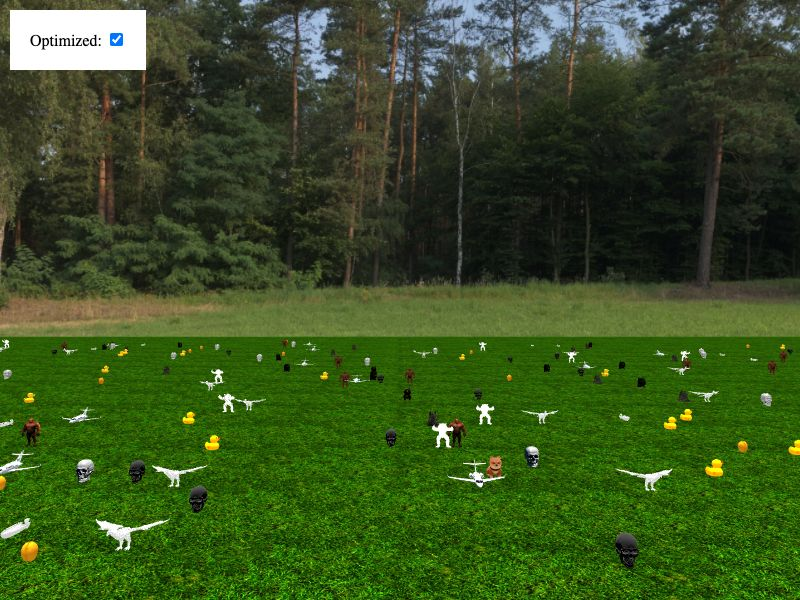
\includegraphics[width=0.8\columnwidth]{resultate/screenshotdemoapplication.jpg}
  \caption{Testapplikation}
  \label{fig:demoApplication}
\end{figure}

\paragraph{Testumgebung}
Um während den Tests möglichst faire Bedingungen zu gewährleisten, wird die Maschine zuvor wie bei anderen Benchmarks vorbereitet. Ziel ist es, Seiteneffekte zu minimieren. Für diesen Benchmark wurden deshalb die Instruktionen von \e{Tracer Bench} zur Behebung von Rauschen befolgt.
\cite{tracerBenchNoiseMitigation}

\paragraph{Analyse der Daten}
Um eine zuverlässige Aussage treffen zu können, wird der Vorgang mehrfach wiederholt. Für jeden Durchlauf wird der Median der \e{\gls{FPS}} Daten berechnet.
Anschliessend wird die Varianz der \e{\gls{FPS}} für die unoptimierten respektive optimierten Werte berechnet. Die Varianz dient als Kennzahl, um eine Signifikanz der Daten nachweisen zu können.

\subparagraph{Konfidenzintervall}
Die Signifikanz wird mithilfe eines statistischen Konfidenzintervalls nachgewiesen. Hierfür wird der Durchschnitt aller Mediane verwendet, zusätzlich wird ein Konfidenzintervall von 95\% gewählt. Es wird gewährleistet, dass das Resultat des Benchmarks verlässlich ist und für einen Vergleich verwendet werden kann.

\subsection{Auswertung}
\label{chap:benchmarkResults}

Der Benchmark wurde auf einer Maschine mit moderner Grafikkarte ausgeführt. Die Resultate zeigen einen klaren Unterschied zwischen der unoptimierten und optimierten Version. So ist die Zeit für das Laden der Modelle zwar geringfügig länger, die Zahl der \e{Render Loop} Iterationen und insbesondere der \e{FPS} geben eine klare Auskunft. Unter Berücksichtigung des berechneten Konfidenzintervalls wird das Resultat als signifikant erachtet. Diese These wird auch durch eine einfache Kontrolle mit dem Auge belegt - die Anzahl \e{FPS} unterscheidet sich merkbar.

Somit ist es möglich einen Nutzen für bestimmte anspruchsvolle 3D-Visualisierungen zu generieren.